\section{Giới thiệu}
\begin{enumerate}
    \item []\hspace*{0.7cm}Trong phần này, chúng tôi sẽ mô tả chi tiết các kết quả đạt được từ việc áp dụng công cụ Selenium để thu thập dữ liệu từ trang web chứng khoán simplize.vn. Quá trình thực hiện, từ thu thập đến phân tích dữ liệu, được trình bày cụ thể cùng với các kết quả thu thập được. Nhờ các dữ liệu này, nhóm nghiên cứu đã phân tích xu hướng cổ phiếu và đánh giá mức độ hiệu quả của việc sử dụng Selenium trong việc tự động hóa quy trình thu thập dữ liệu.
\end{enumerate}

\section{Kết quả thu thập dữ liệu}
\begin{enumerate}
    \item []\hspace*{0.7cm}Dữ liệu được thu thập từ trang web simpile.vn bao gồm các thông tin như: ngày, giá mở cửa, giá cao nhất, giá thấp nhất, giá đóng cửa, thay đổi giá, \% thay đổi, khối lượng và hồ sơ doanh nghiệp. Sau khi hoàn tất quá trình thu thập, tổng số mã lấy được là \textbf{80 mã} trong nhóm ngành tài chính và số ngày lấy được của từng mã là \textbf{60 ngày}.
    
    \item []\hspace*{0.7cm}Dữ liệu sẽ được đưa vào MongoDB và được lưu trữ để phục vụ các bước phân tích cho tương lai.

    
\end{enumerate}
\section{Phân tích dữ liệu}
\begin{enumerate}
    \item []
    \begin{figure}[h]
        \centering
        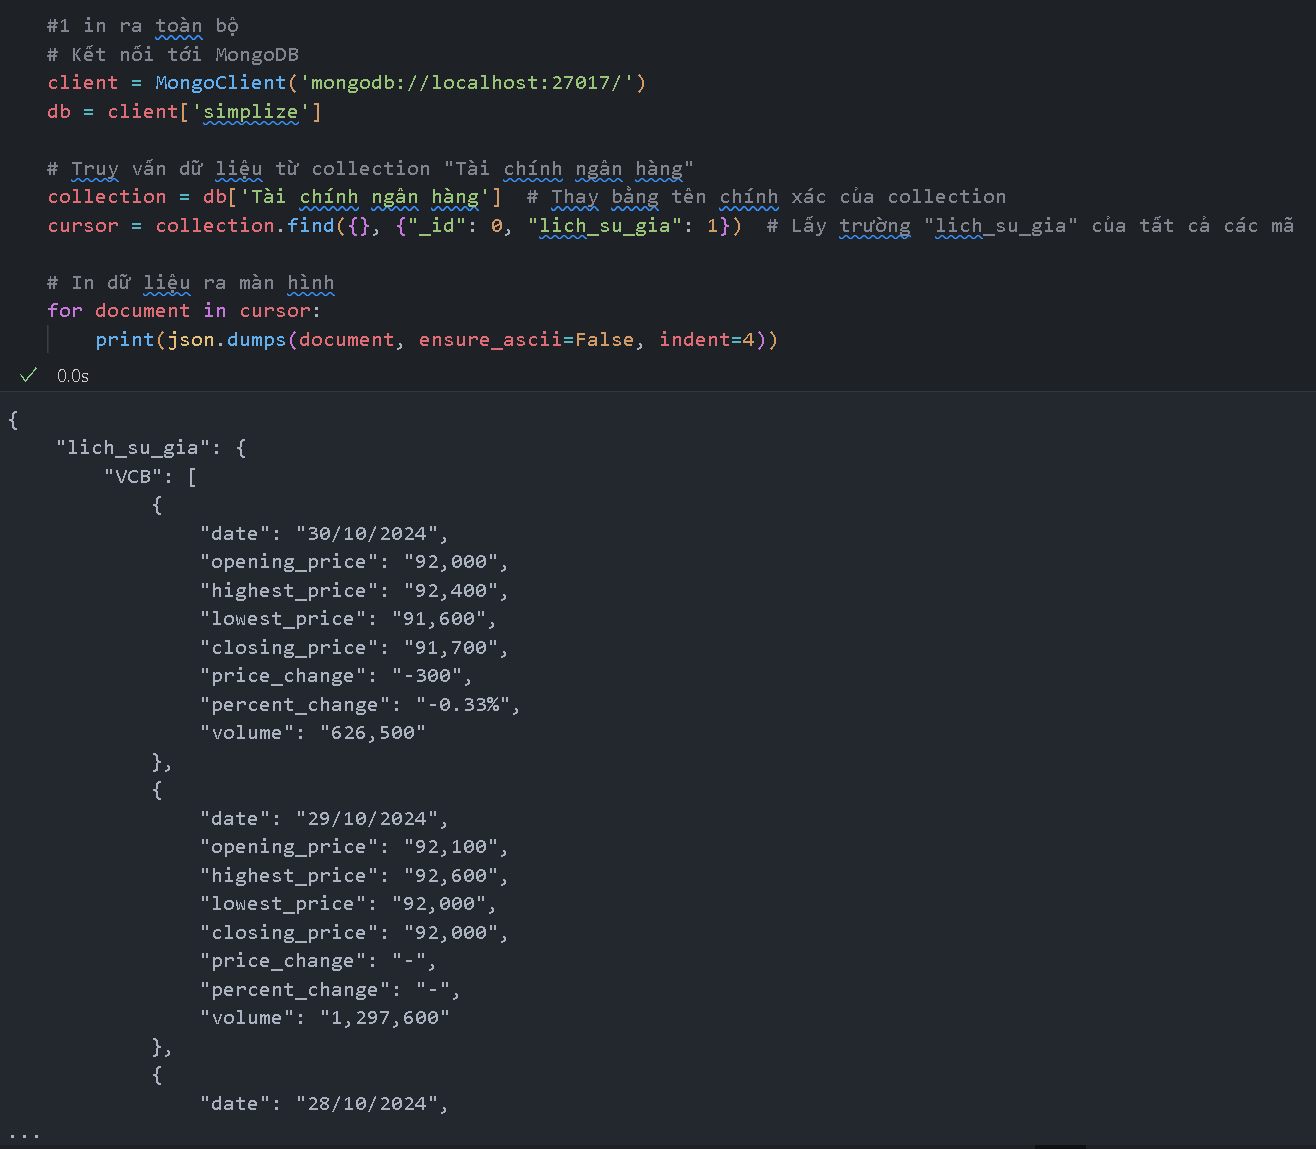
\includegraphics[width=0.8\linewidth]{img/img_query/1.png}
        \caption{In ra toàn bộ}
        \label{fig:1_query}
    \end{figure}
\end{enumerate}
\newpage
\begin{enumerate}
    \item []
    \begin{figure}[h]
        \centering
        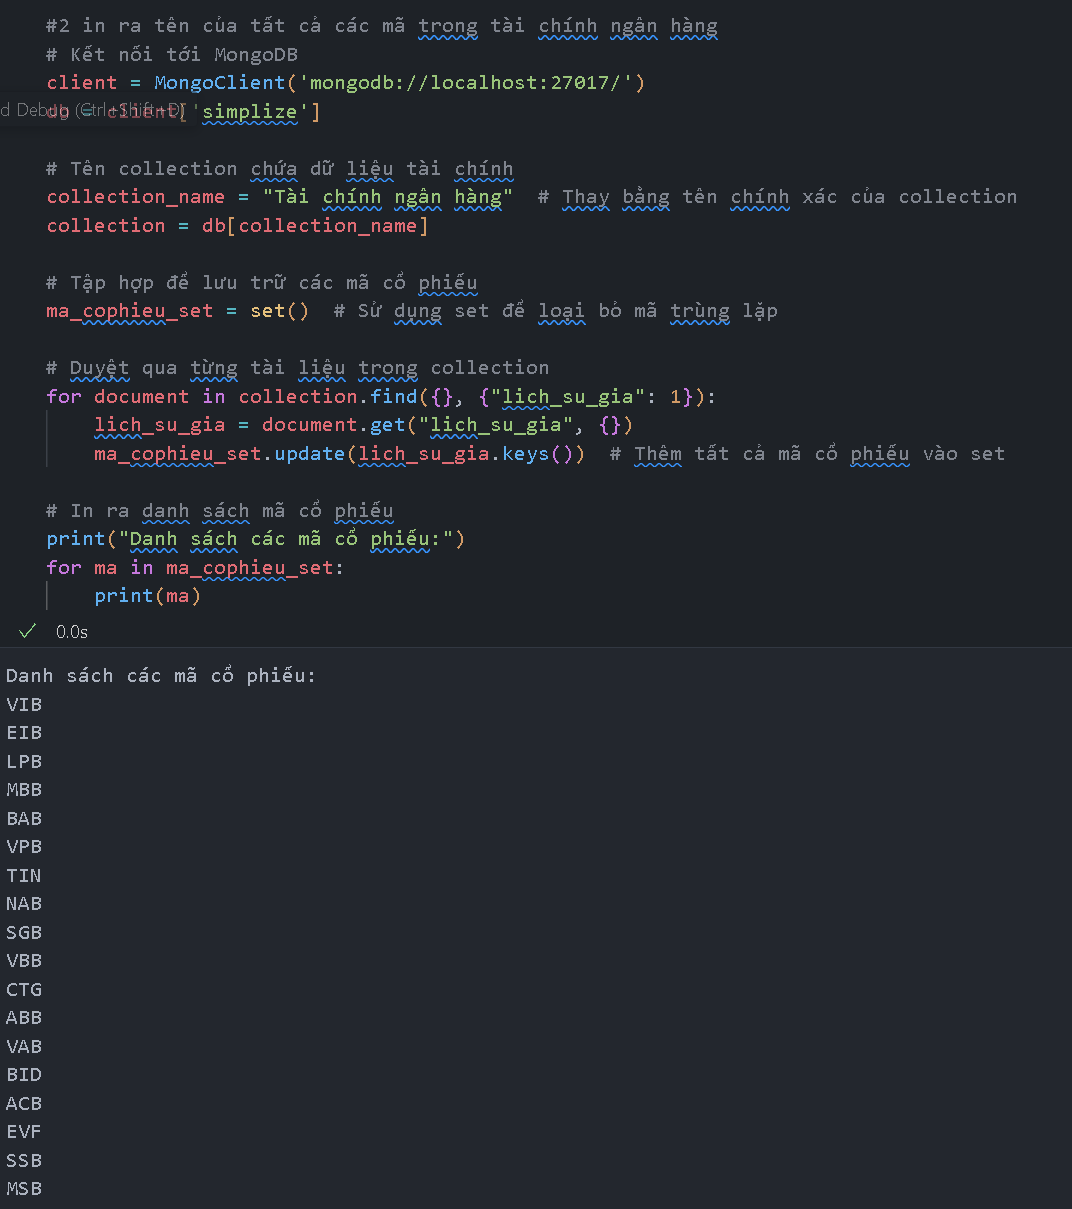
\includegraphics[width=0.8\linewidth]{img/img_query/2.png}
        \caption{in ra tên của tất cả các mã trong tài chính ngân hàng}
        \label{fig:2_query}
    \end{figure}
\end{enumerate}
\newpage
\begin{enumerate}
    \item []
    \begin{figure}[h]
        \centering
        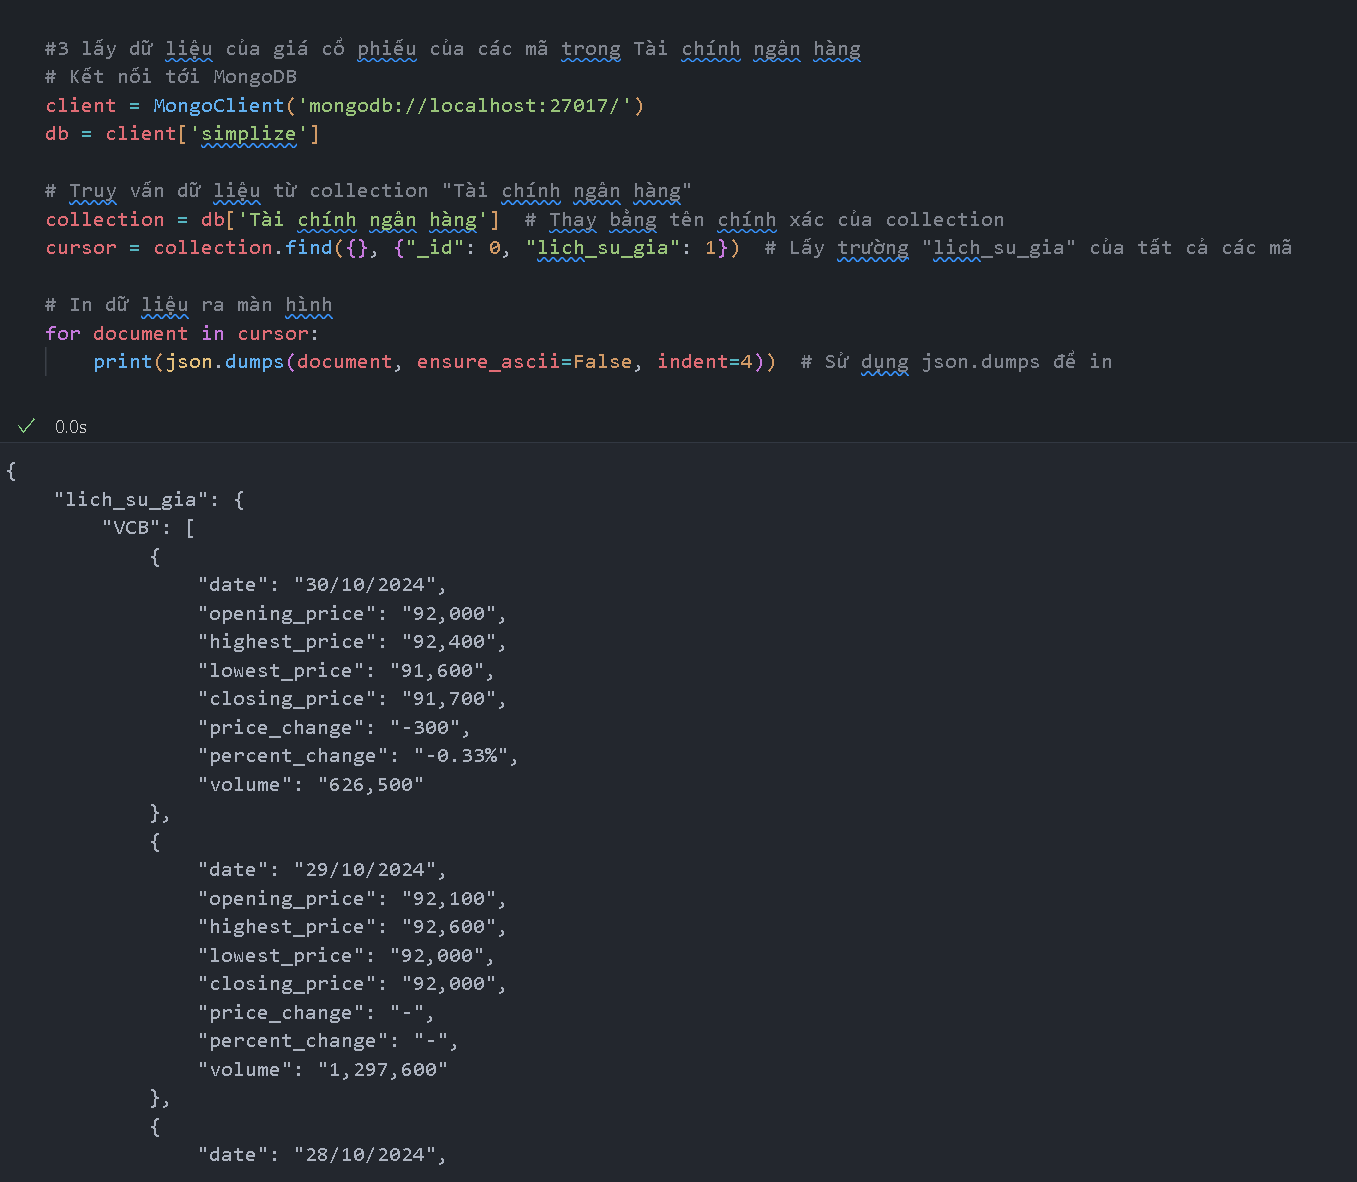
\includegraphics[width=0.8\linewidth]{img/img_query/3.png}
        \caption{lấy dữ liệu của giá cổ phiếu của các mã trong Tài chính ngân hàng}
        \label{fig:3_query}
    \end{figure}
\end{enumerate}
\newpage
\begin{enumerate}
    \item []
    \begin{figure}[h]
        \centering
        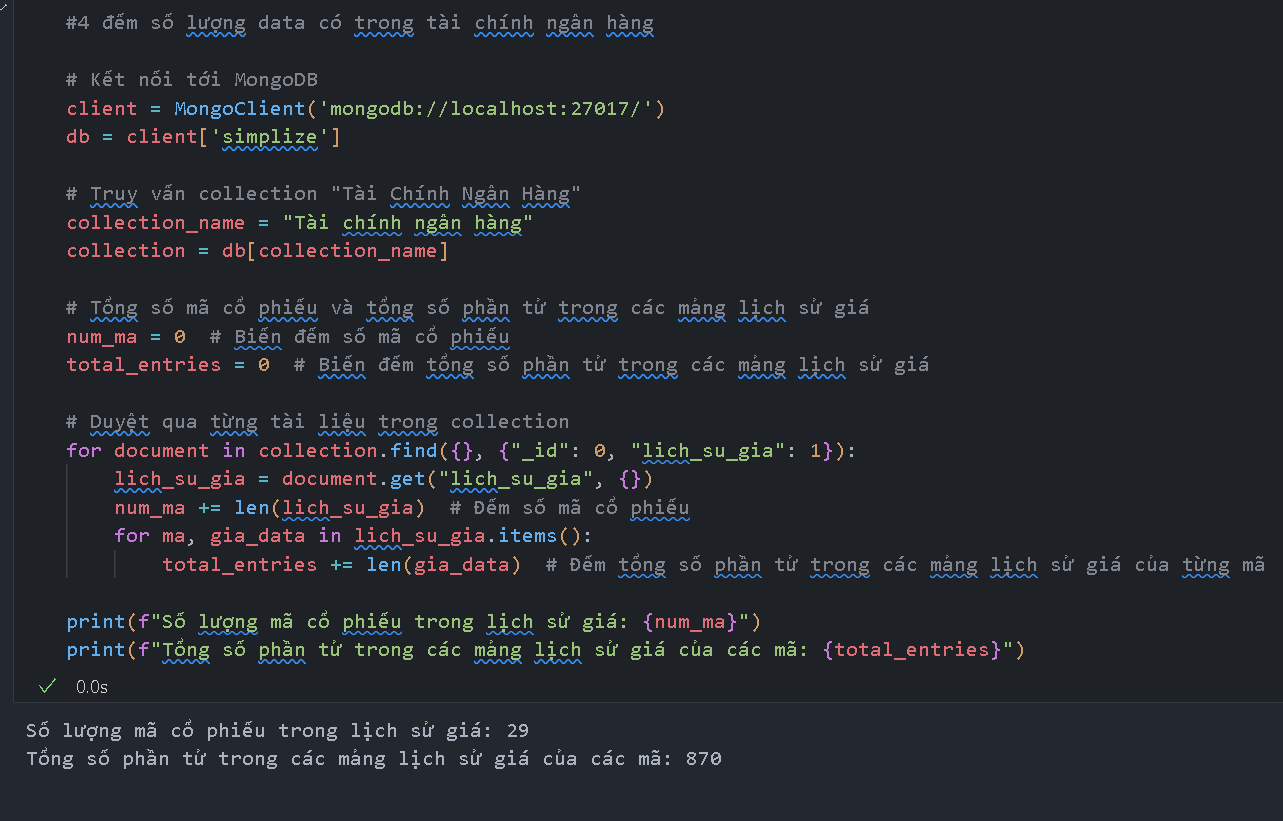
\includegraphics[width=0.8\linewidth]{img/img_query/4.png}
        \caption{đếm số lượng data có trong tài chính ngân hàng}
        \label{fig:4_query}
    \end{figure}
\end{enumerate}
\newpage
\begin{enumerate}
    \item []
    \begin{figure}[h]
        \centering
        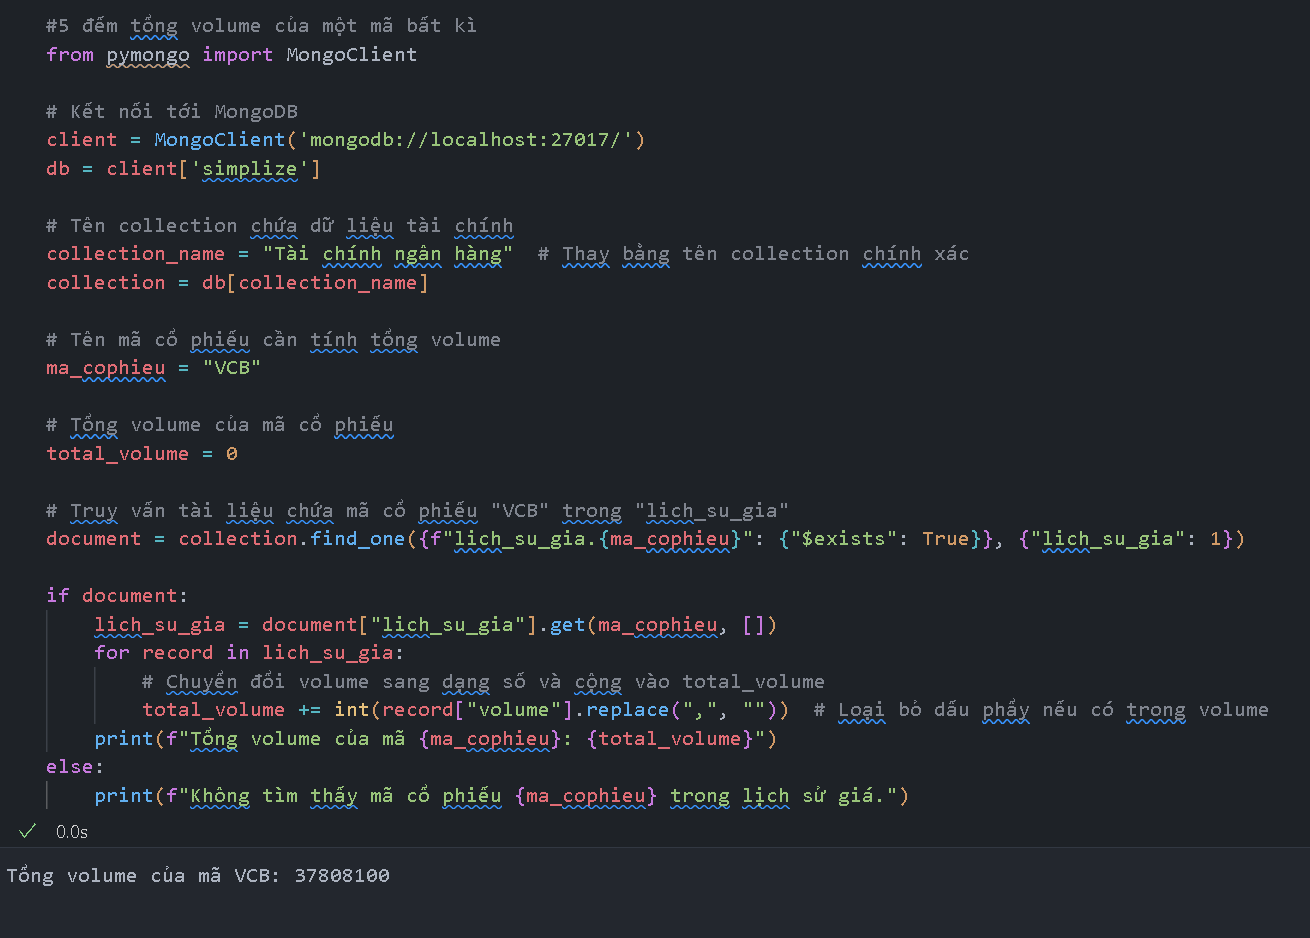
\includegraphics[width=0.8\linewidth]{img/img_query/5.png}
        \caption{đếm tổng volume của một mã bất kì}
        \label{fig:5_query}
    \end{figure}
\end{enumerate}
\newpage
\begin{enumerate}
    \item []
    \begin{figure}[h]
        \centering
        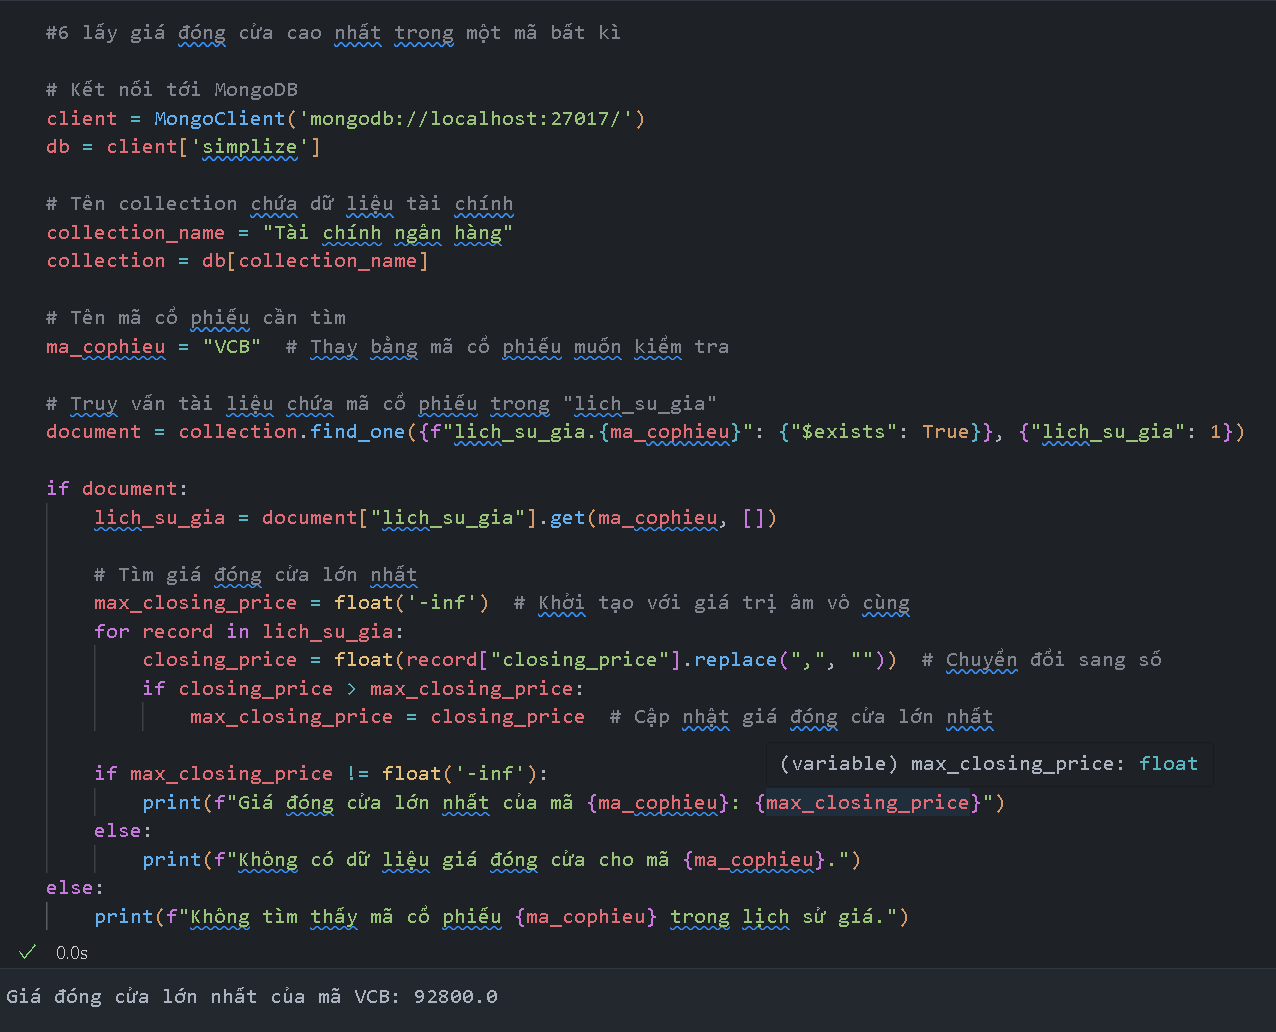
\includegraphics[width=0.8\linewidth]{img/img_query/6.png}
        \caption{đếm tổng volume của một mã bất kì}
        \label{fig:6_query}
    \end{figure}
\end{enumerate}
\newpage
\begin{enumerate}
    \item []
    \begin{figure}[h]
        \centering
        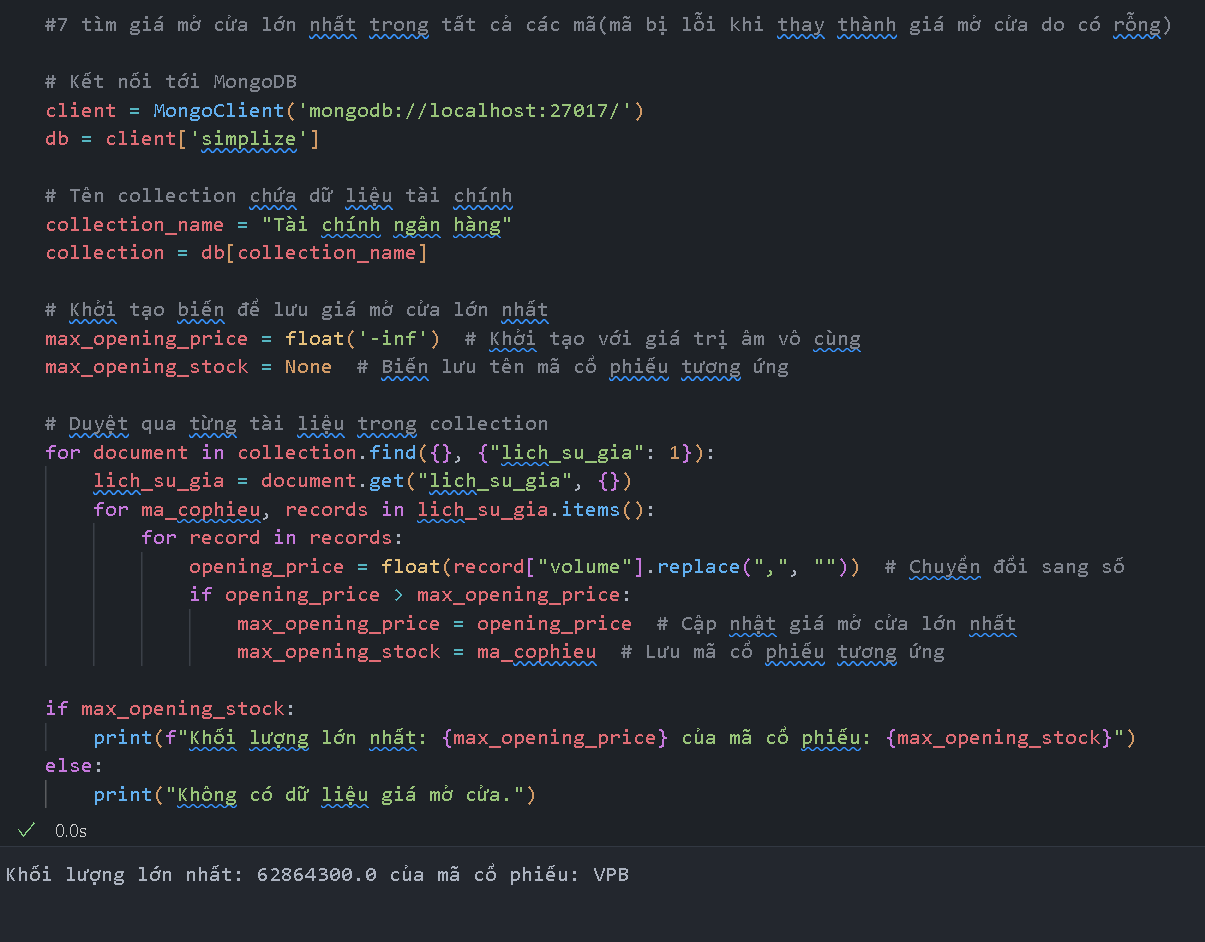
\includegraphics[width=0.8\linewidth]{img/img_query/7.png}
        \caption{tìm giá mở cửa lớn nhất trong tất cả các mã(mã bị lỗi khi thay thành giá mở cửa do có rỗng)
}
        \label{fig:7_query}
    \end{figure}
\end{enumerate}
\newpage
\begin{enumerate}
    \item []
    \begin{figure}[h]
        \centering
        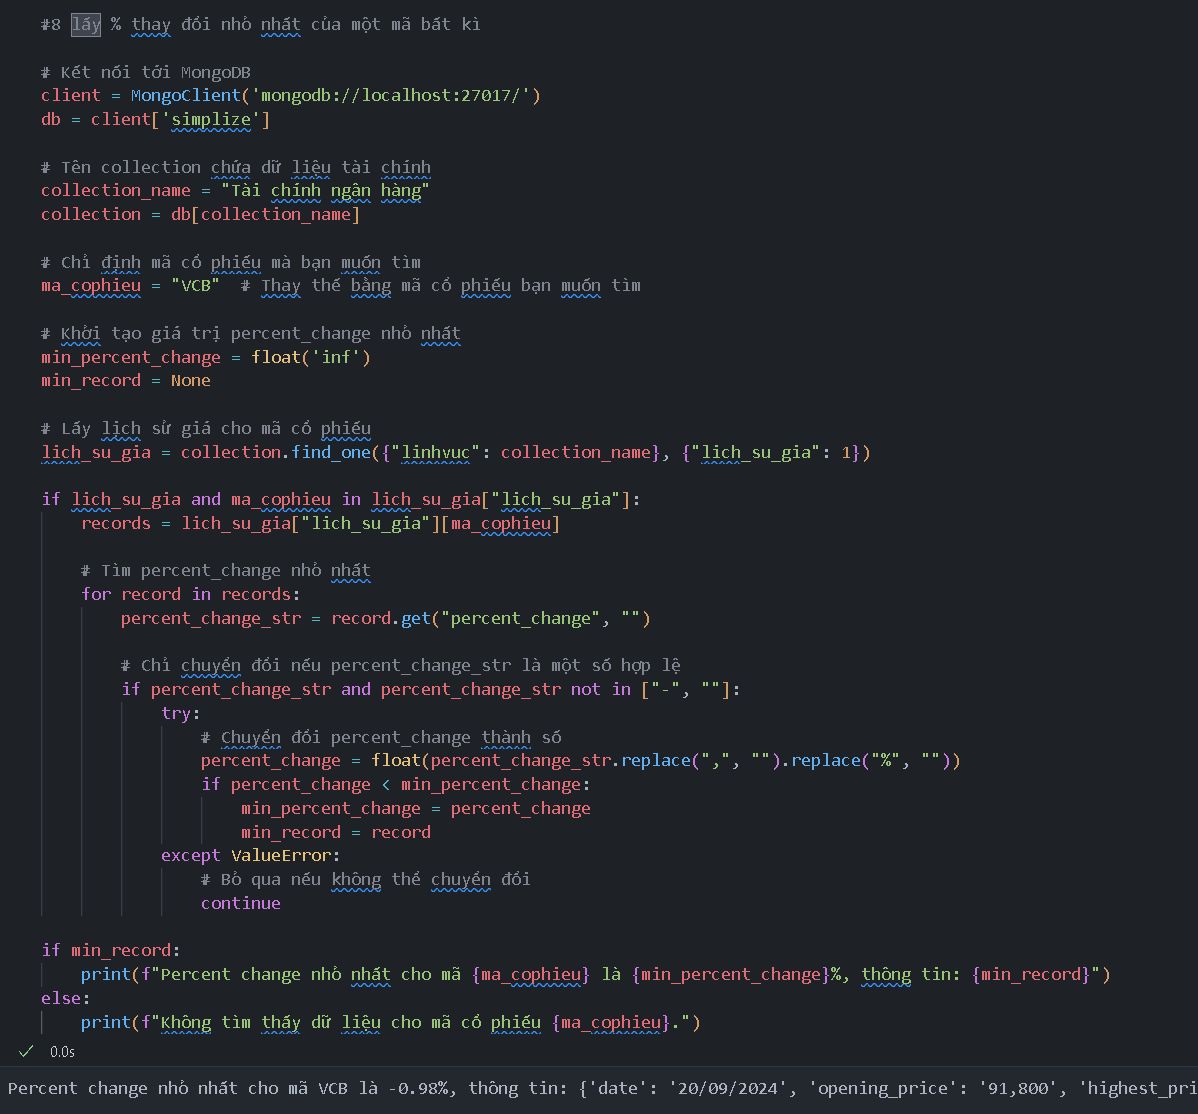
\includegraphics[width=0.8\linewidth]{img/img_query/8.png}
        \caption{lấy \% thay đổi nhỏ nhất của một mã bất kì
}
        \label{fig:8_query}
    \end{figure}
\end{enumerate}
\newpage
\begin{enumerate}
    \item []
    \begin{figure}[h]
        \centering
        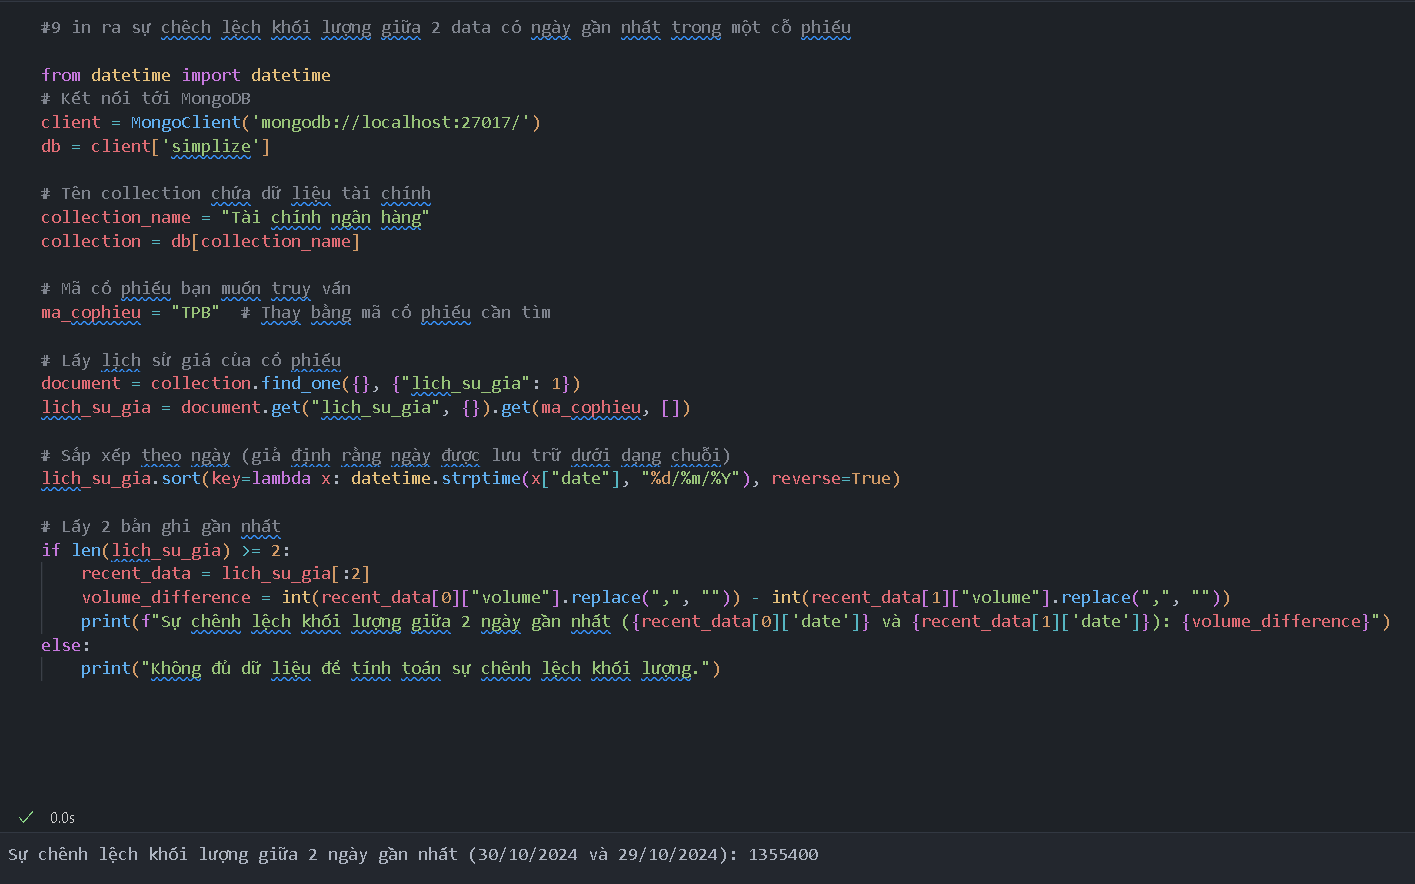
\includegraphics[width=0.8\linewidth]{img/img_query/9.png}
        \caption{in ra sự chêch lệch khối lượng giữa 2 data có ngày gần nhất trong một cỗ phiếu
}
        \label{fig:9_query}
    \end{figure}
\end{enumerate}
\newpage
\begin{enumerate}
    \item []
    \begin{figure}[h]
        \centering
        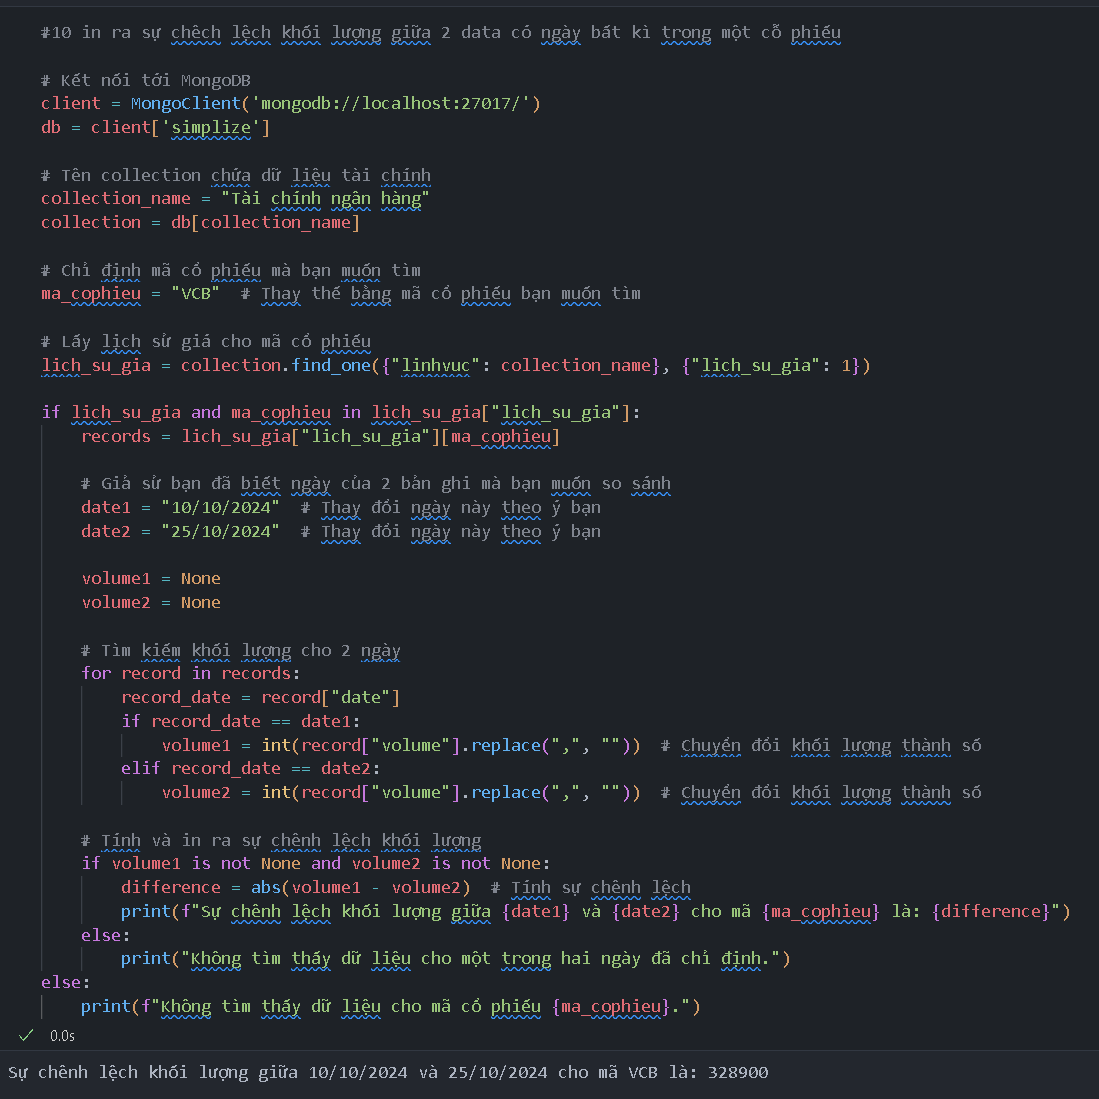
\includegraphics[width=0.8\linewidth]{img/img_query/10.png}
        \caption{in ra sự chêch lệch khối lượng giữa 2 data có ngày bất kì trong một cỗ phiếu
}
        \label{fig:10_query}
    \end{figure}
\end{enumerate}
\newpage
\begin{enumerate}
    \item []
    \begin{figure}[h]
        \centering
        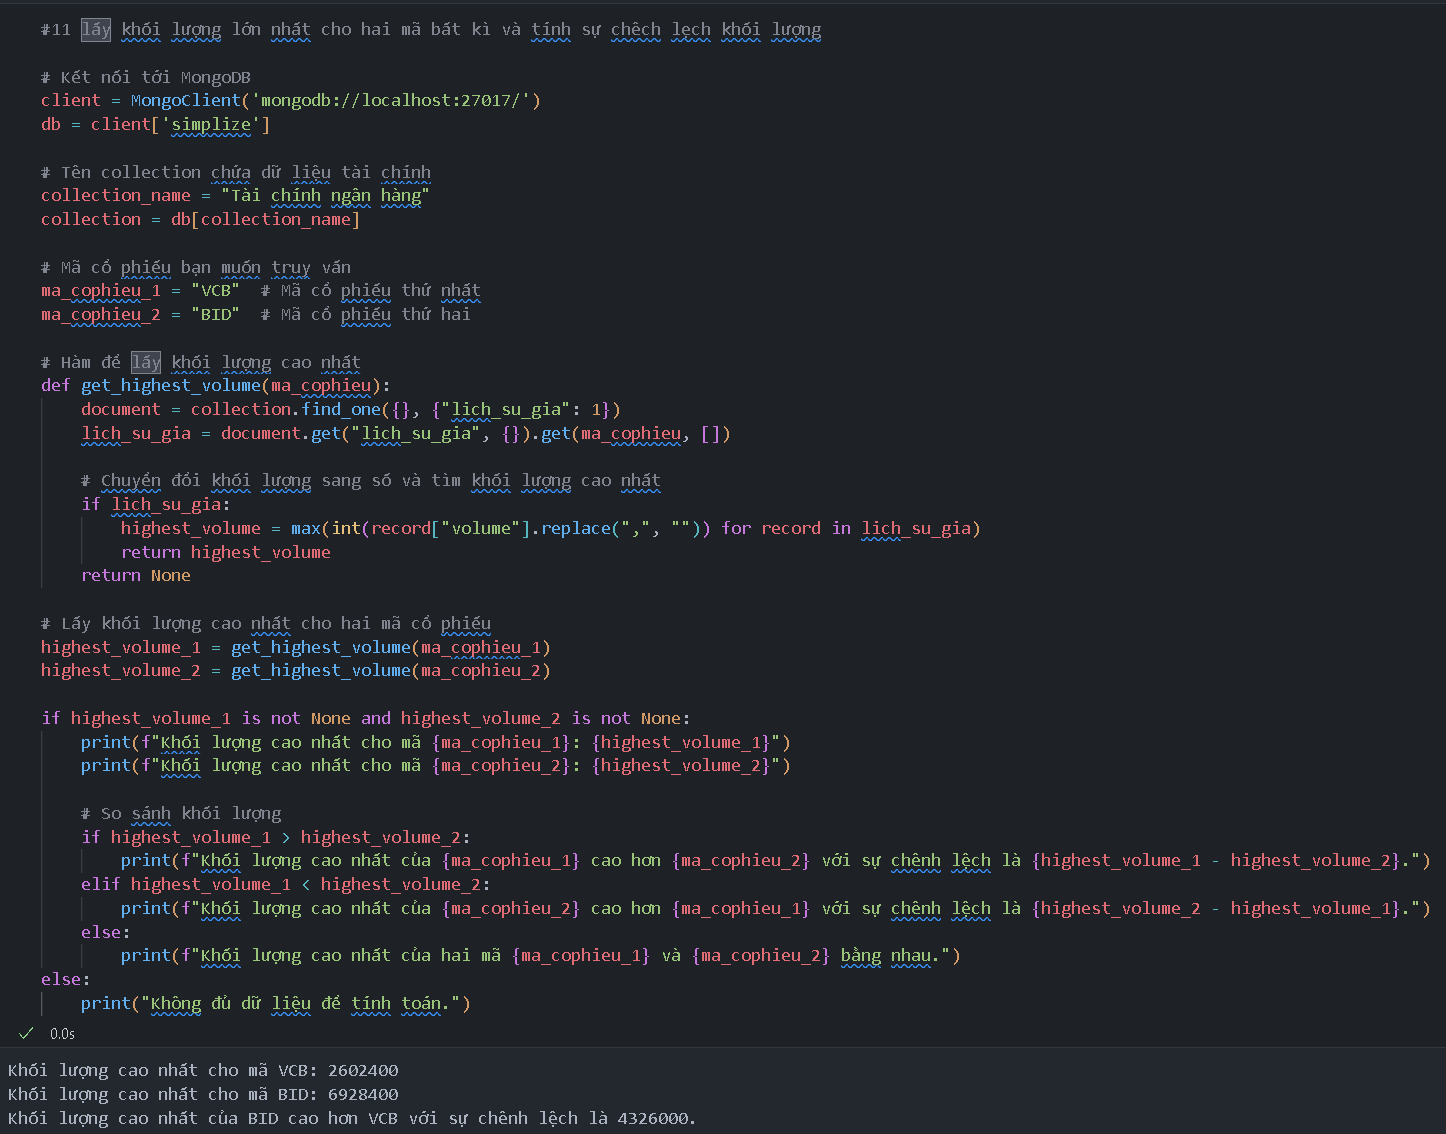
\includegraphics[width=0.8\linewidth]{img/img_query/11.png}
        \caption{lấy khối lượng lớn nhất cho hai mã bất kì và tính sự chêch lẹch khối lượng
}
        \label{fig:11_query}
    \end{figure}
\end{enumerate}
\newpage
\begin{enumerate}
    \item []
    \begin{figure}[h]
        \centering
        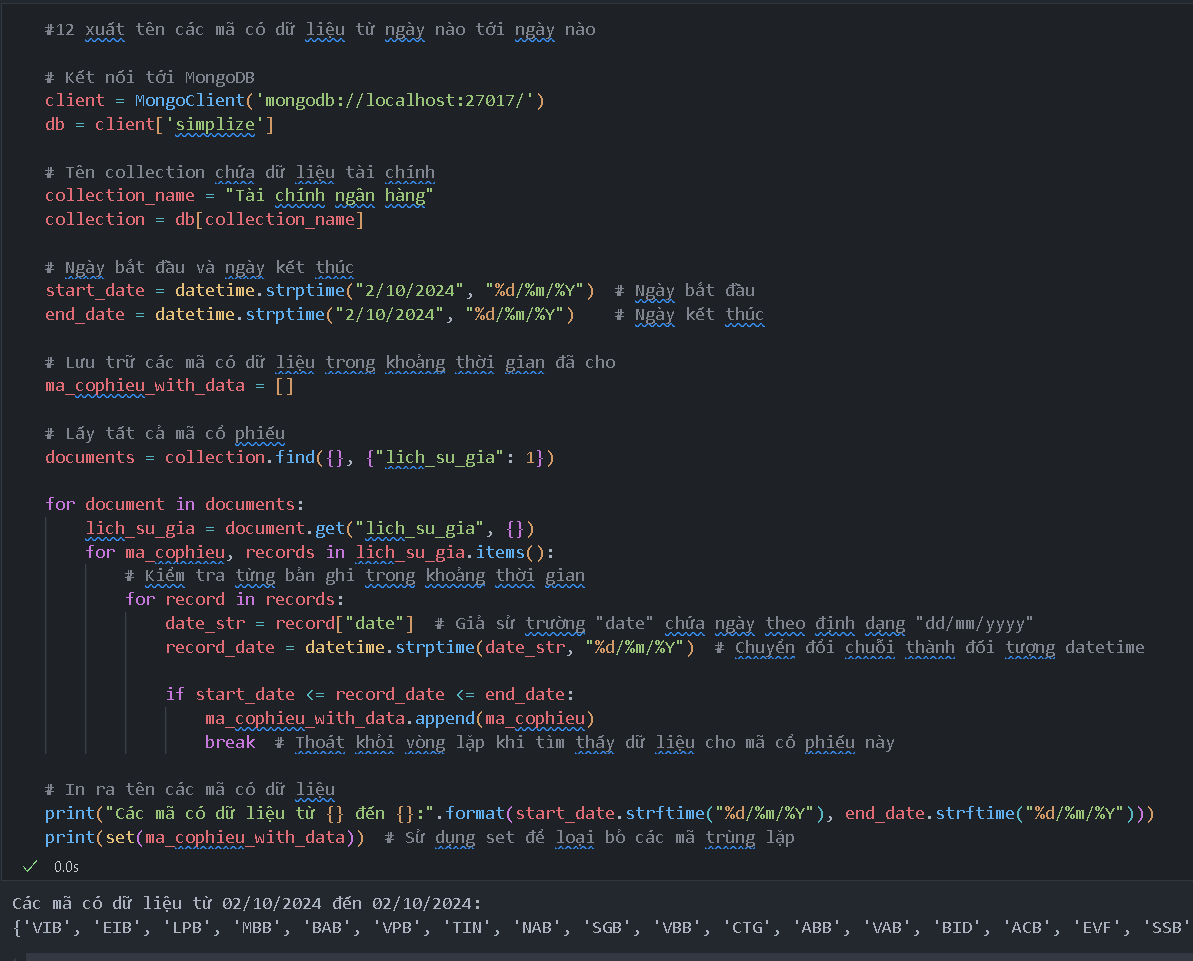
\includegraphics[width=1.0\linewidth]{img/img_query/12.png}
        \caption{xuất tên các mã có dữ liệu từ ngày nào tới ngày nào
}
        \label{fig:12_query}
    \end{figure}
\end{enumerate}
\newpage
\section{Đánh giá hiệu suất Selenium}
\begin{enumerate}
    \item []\hspace*{0.7cm}Qua quá trình thực nghiệm, chúng tôi đã đánh giá hiệu quả của\\Selenium trong việc thu thập dữ liệu từ trang web simplize.vn. Kết quả cho thấy Selenium là một công cụ mạnh mẽ và linh hoạt, phù hợp cho việc thu thập dữ liệu từ các trang có nội dung động và yêu cầu tương tác với người dùng.
    \begin{itemize}[left=0.5cm]
    \item [$\bullet$]\textbf{Hiệu suất:}Selenium có khả năng thu thập dữ liệu từ 80 mã chứng khóa với tốc độ khoảng 1 mã/phút, giúp tiết kiệm đáng kể thời gian so với phương pháp thu thập thủ công. Toàn bộ quá trình thu thập dữ liệu cho 80 mã tốn khoảng 70 phút.
    \item [$\bullet$]\textbf{Khả năng xử lý lỗi:}Trong quá trình thu thập, Selenium có thể tự động xử lý các sự cố về kết nối và các yêu cầu không thành công. Tỷ lệ lỗi phát sinh rất thấp, chỉ khoảng 0.1\% trên tổng số yêu cầu được gửi đi.
    \item [$\bullet$]\textbf{Tính chính xác:}Dữ liệu được thu thập có độ chính xác cao, với tỷ lệ thành công vượt quá 98\% mà không gặp phải lỗi nào.
    \end{itemize}
\end{enumerate}

\section{Các khó khăn và hạn chế}
\begin{enumerate}
    \item []\hspace*{0.7cm}Mặc dù Selenium đã mang lại hiệu quả cao trong việc thu thập dữ liệu, chúng tôi cũng gặp phải một số thách thức đáng lưu ý:
    
\begin{itemize}[left=0.5cm]
    \item [$\bullet$]\textbf{Tốc độ tải trang:} Do Selenium tương tác trực tiếp với trình duyệt và phải xử lý toàn bộ nội dung trang, quá trình thu thập dữ liệu từ những trang web có lượng nội dung lớn hoặc tốc độ tải chậm có thể kéo dài đáng kể, làm giảm hiệu suất so với các công cụ nhẹ hơn như Scrapy.
    
    \item [$\bullet$]\textbf{Quản lý phiên (session):} Một số trang web yêu cầu duy trì trạng thái phiên liên tục, và điều này đòi hỏi việc thiết lập phiên trong Selenium phải được thực hiện chính xác. Nếu không, quá trình thu thập có nguy cơ bị gián đoạn, dẫn đến mất mát hoặc sai sót dữ liệu.
\end{itemize}

\end{enumerate}
\section{Kết luận}
\begin{enumerate}
    \item []\hspace*{0.7cm}Chương này đã trình bày các kết quả thực nghiệm thu thập và phân tích dữ liệu từ trang web chứng khoán simplize.vn bằng công cụ Selenium. Kết quả cho thấy Selenium là một công cụ mạnh mẽ cho việc tự động thu thập dữ liệu từ các trang web động, đặc biệt là khi xử lý nội dung được tải qua JavaScript. Mặc dù quá trình thu thập có thể chậm hơn do phải tải toàn bộ trang, nhưng lợi ích của Selenium nằm ở khả năng xử lý các trang web phức tạp và đảm bảo thu thập đầy đủ dữ liệu, điều mà các công cụ khác khó thực hiện. Vì vậy, mặc dù thời gian thực thi có thể dài hơn, Selenium vẫn mang lại hiệu quả cao trong các tình huống cần tương tác trực tiếp với nội dung trang.
\end{enumerate}

